\Section{natlog-mono}{Monotonicity Calculus}

%
% Intro with Algebra
%
We begin this section by reviewing monotonicity in its familiar context:
  monotonicity of algabraic functions.
For example, $f(x) = e^x - 1$ is a \textit{monotone} function -- as we increase $x$,
  the value of $f(x)$ monotonicially increases.
A function may also be \textit{antitone}: $f(x) = e^{-x}$ is antitone, since 
  the value of $f(x)$ decreases monotonically as $x$ increases.
Lastly, a function can be \textit{nonmonotone} -- distinct from antitone -- if
  it is neither monotone nor antitone.

Visually, the plots below show a monotone function ($e^x - 1$) and an antitone 
  function ($e^{-x}$).
We will appeal to analogous visualizations when we move towards working with
  language.

\begin{center}
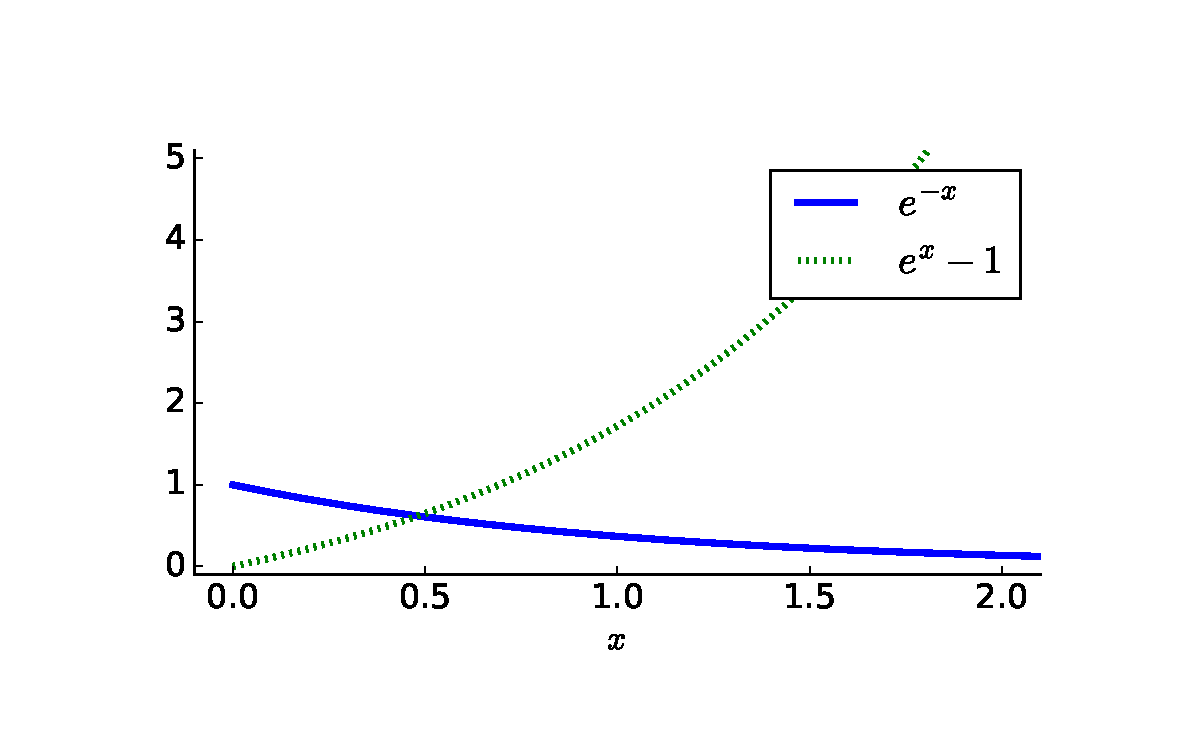
\includegraphics[height=7cm]{img/monotonicity_math.pdf}
\end{center}


% Sales Pitch
Monotonicity is an appealing tool because it lets us reason about functions
  without having to evaluate them.
To illustrate, we can define an arbitrarily complex function $f : \R \rightarrow \R$,
  which we are told is monotone.
Without evaluating the function, we are able to conclude that
  $f(x + 1) > f(x)$.
This is precisely the type of tool we would like to use to manipulate language:
  constructing a concrete interpretation of language -- like evaluating 
  a complex function -- is at best undesirable and at worst impossible.
However, if we know some properties about the ``monotonicity'' of the language,
  we can manipulate the text such that we preserve some key relations
  between the original and our mutated text -- analogous to the greater-than
  relation in our algebraic example.

In fact, this analog is much more direct than it may at first appear:
  monotonicity calculus reasons about the functions defined in 
  \refsecs{natlog-denotations-other}{natlog-denotations-quantifiers}.
The remainder of this section will explore how to apply monotonicity to
  the denotational semantics in \refsec{natlog-denotations},
  and then introduce reasoning about exclusion (\refsec{natlog-mono-exclusion}).
The section will conclude by introducing the notion of \textit{polarity},
  and exploring how to compose monotone functions in a sentence.



%
% Monotonicity in Language
%
\Subsection{natlog-mono-general}{Monotonicity in Langugage}

In generality, a monotone function is a function between partially-ordered sets
  that preserves the given order.
For a function $f$ with domain $\bX$ and range $\bY$, we define a partial order over
  $\leq_X$ and $\leq_Y$.
This function is monotone iff:

\begin{equation}
  \forall x_1, x_2 \in \bX ~~ \textrm{such that} ~~ x_1 \leq_X x_2; ~~  f(x_1) \leq_Y f(x_2)
\end{equation}

We note from \refsec{natlog-denotations} that, by and large, sentences 
  are constructed by composing one or more functions (e.g., verbs, operators).
To reason about whether these functions are monotone (or, by extenstion, antitone),
  we need to show that each of our domains forms a partial order we can define
  monotonicity against.

First: the domain of noun denotations: $\sD_e$ (or, $e$).
We define our partial order $\leq_e$ to be the subset operator: $\subseteq$.
That is, if the denotation of a word is completely contained in the denotation of
  another word, we consider the first word to be ``less than'' the second.
This is intuitively encoding hypernymy as a partial order.
For example, $\llbracket cat \rrbracket$ $\leq_e$ $\llbracket feline \rrbracket$ because
  any entity which is a cat is also necessarily a feline.

Second: the domain of truth values: $\sD_t$ (or, $t$).
Here, we axiomatically define a partial order $\leq_t$ to be:\footnote{
    The elegance of the interpretation of false as the empty set and true as a singleton
    set becomes clear here: we can define the partial order over truth values to be the same
    subset operator as the partial order over noun denotations.
    }

\begin{align*}
  false &\leq_t false \\
  false &\leq_t true \\
  true &\leq_t true \\
\end{align*}

The very important observation to make at this point is that
  \textbf{the partial order $\leq_t$ corresponds exactly to the material conditional $\supset$}.
So, for any two propositions $A$ and $B$, $A$ entails $B$ ($A \supset B$) is the same
  as $A \leq_t B$.
This is the key insight tying together the concepts of monotonicity and entailment.
We also point out the unfortunate fact that the symbol for the material conditional
  is the same as the superset symbol, which would seem to evoke ``greater than'' rather
  than the ``less than'' it actually corresponds to.
Unfortunately, I do not yet have the political capital to redefine either of these
  symbols.

Lastly: we must define a partial order over our inductively defined function types.
We adopt the definition that a function is less than another function if, for all
  values in the domain of the functions, the value of the first function is less than
  the value of the second.
Formally: for two functions $f$ and $g$ with the same domain and range $\bX \rightarrow \bY$,
  we say $f \leq_f g$ iff:

\begin{equation}
  \forall x \in \bX; ~~ f(x) \leq_Y g(x)
\end{equation}

For the remainder of this thesis, we will collapse all of these partial orders
  -- $\leq_e$, $\leq_t$, and $\leq_f$ -- into
  a single symbol: \forward.



% Monotonicity is entailment-preserving
\paragraph{Monotonicity is Entailment-Preserving}
An important insight from the partial orders above is that our partial order
  over truth values corresponds exactly to entailment.
Although ``entailment'' is not particularly well-defined for the other denotation
  types (i.e., does \ww{cat} entail \ww{animal}?), for the purposes of monotonicity
  calculus and natural logic we will take the symbol \forward\ to be entailment.\footnote{
    This is, again, not to be confused with the symbol for entailment in propositional
    logic: $\supset$.
  }
By extension, we can define $A \reverse B$ to mean that $B \forward A$, and define
  \equivalent\ to be equivalence.
That is to say, $A \equivalent B$ is the same as $A \forward B$ and $B \forward A$.

This means that monotone functions are entailment preserving.
If a sentence is true, and the function used to construct its denotation (i.e., truth)
  is monotone with respect to the denotation of a word, then replacing that word with
  another word whose denotation is a superset of the original word will maintain
  the truth of the sentence.

Taking a concrete example: \ww{all} (a function $e \rightarrow (e \rightarrow t)$)
  is antitone in its first argument and monotone in its second.
So, the sentence \ww{all cats drink milk} is antitone with respect to \ww{cats} and
  monotone with respect to \ww{drink milk}.
Furthermore, we know that 
  $\llbracket drink ~ milk\rrbracket \forward \llbracket drink~dairy\rrbracket$
  because $\llbracket milk\rrbracket \forward \llbracket dairy\rrbracket$.
Therefore, by the definition of monotonicity, we can replace \ww{drink milk} with
  \ww{drink dairy} and the resulting sentence (\ww{all cats drink dairy})
  is guaranteed to be true if the original sentence was true.

The fact that quantifiers and other operators in natural language have this
  property of monotonicity is wonderfully convenient.
Grounding an interpretation for \ww{all cats drink milk} would be rather
  difficult in the general case -- and certainly difficult for longer utterances.
But by appealing to the monotonicity of quantifiers, we do not need to ground
  the sentence to run an entailment proof on it.

Antitone functions behave analogously to monotone functions, but with the 
  direction of the lexical mutation reversed.
For example, if \ww{all cats drink milk}, we can infer that 
  \ww{all kittens drink milk} because 
  $\llbracket cat \rrbracket \reverse \llbracket kitten\rrbracket$.

Like the visualization with monotone algebreic functions earlier in the section,
  we can visualize monotonicity over denotations.
In the chart below, the $x$ axis is an ordering over denotations.\footnote{
    In general this is a partial order; however, partial orders are difficult
    to plot on an axis.
    }
The $y$ axis is the ordering over truth values.
We are plotting two functions: \ww{all $x$ drink milk} -- antitone in $x$; and
  \ww{some $x$ bark} -- monotone in $x$:

\begin{center}
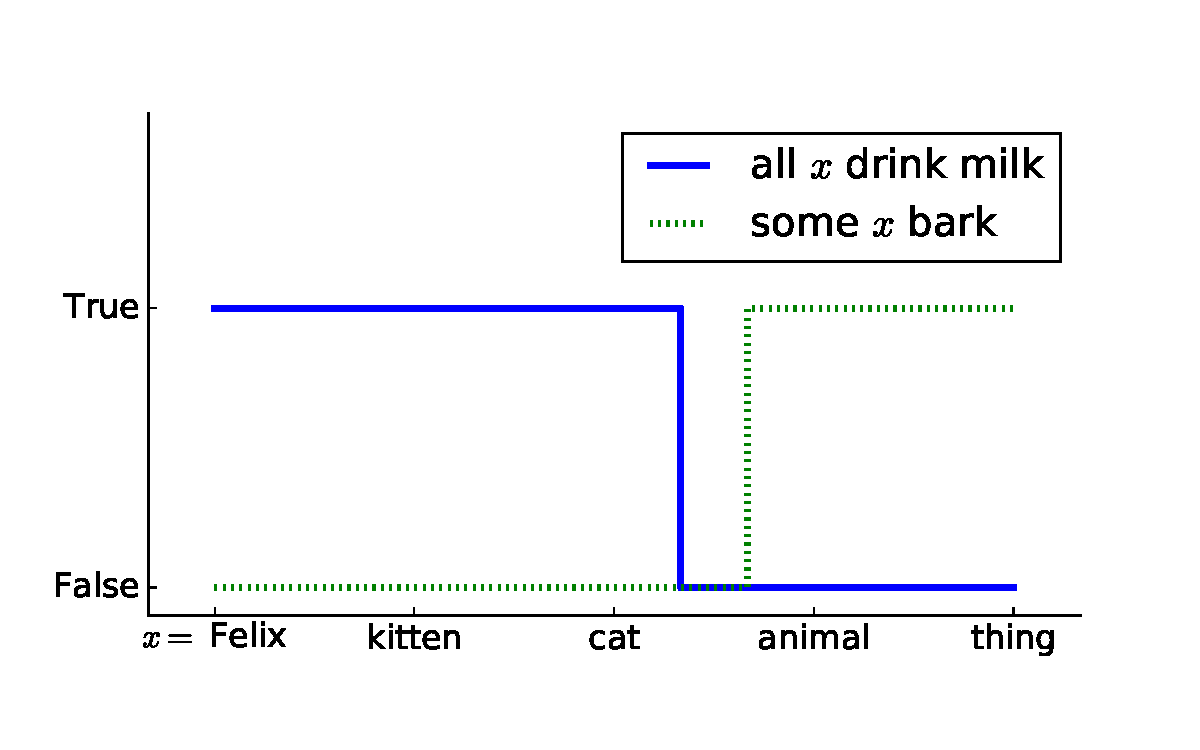
\includegraphics[height=7cm]{img/monotonicity_lex_all.pdf}
\end{center}

% Back to proof theory for a bit
\paragraph{Monotonicity Calculus as a proof theory}
At this point, we can begin looking at monotonicity calculus as the sort of natural
  logic proof system we demonstrated at the beginning of the chapter.
For example, our inference from \ww{the cat ate a mouse} to 
  \ww{the carnivore ate an animal} could be formally justified with the following proof.
We note that the quantifier \ww{the} -- like \ww{some} -- is monotone in both
  of its arguments.

\[
\begin{nd}
\hypo {1} {\ww{The cat ate a mouse.}}
\have {2} {\ww{The cat ate a rodent.}}         \by{\denote{mouse} \forward\ \denote{rodent}}{1}
\have {3} {\ww{The cat ate an animal.}}        \by{\denote{rodent} \forward\ \denote{animal}}{2}
\have {4} {\ww{The feline ate an animal.}}     \by{\denote{cat} \forward\ \denote{feline}}{3}
\have {5} {\ww{The carnivore ate an animal.}}  \by{\denote{carnivore} \forward\ \denote{animal}}{4}
\end{nd}
\]

However, we still lack the tools to infer that \ww{no carnivore ate an animal} is false
  given our premise.
For this, we need a theory of how to reason with \textit{exclusion} -- which we will
  review in the next section.
Furthermore, our theory currently does not handle nested quantification.
We introduce \textit{Polarity} and the mechanism for propagating monotonicity information
  to determine the ``monotonicty'' of a sentence composed of multiple quantifiers.



%
% Exclusion
%
\Subsection{natlog-mono-exclusion}{Exclusion}
Reasoning with exclusion is an extension of the monotonicity calculus of
  \newcite{key:1991valencia-natlog}, introduced by
  \newcite{key:2008maccartney-natlog} and formalized by
  \newcite{key:2014icard-natlog}.




%
% Polarity
%
\Subsection{natlog-mono-polarity}{Polarity: Composing Monotonicity}
